% Options for packages loaded elsewhere
\PassOptionsToPackage{unicode}{hyperref}
\PassOptionsToPackage{hyphens}{url}
%
\documentclass[
  man,floatsintext]{apa7}
\usepackage{amsmath,amssymb}
\usepackage{iftex}
\ifPDFTeX
  \usepackage[T1]{fontenc}
  \usepackage[utf8]{inputenc}
  \usepackage{textcomp} % provide euro and other symbols
\else % if luatex or xetex
  \usepackage{unicode-math} % this also loads fontspec
  \defaultfontfeatures{Scale=MatchLowercase}
  \defaultfontfeatures[\rmfamily]{Ligatures=TeX,Scale=1}
\fi
\usepackage{lmodern}
\ifPDFTeX\else
  % xetex/luatex font selection
\fi
% Use upquote if available, for straight quotes in verbatim environments
\IfFileExists{upquote.sty}{\usepackage{upquote}}{}
\IfFileExists{microtype.sty}{% use microtype if available
  \usepackage[]{microtype}
  \UseMicrotypeSet[protrusion]{basicmath} % disable protrusion for tt fonts
}{}
\makeatletter
\@ifundefined{KOMAClassName}{% if non-KOMA class
  \IfFileExists{parskip.sty}{%
    \usepackage{parskip}
  }{% else
    \setlength{\parindent}{0pt}
    \setlength{\parskip}{6pt plus 2pt minus 1pt}}
}{% if KOMA class
  \KOMAoptions{parskip=half}}
\makeatother
\usepackage{xcolor}
\usepackage{graphicx}
\makeatletter
\def\maxwidth{\ifdim\Gin@nat@width>\linewidth\linewidth\else\Gin@nat@width\fi}
\def\maxheight{\ifdim\Gin@nat@height>\textheight\textheight\else\Gin@nat@height\fi}
\makeatother
% Scale images if necessary, so that they will not overflow the page
% margins by default, and it is still possible to overwrite the defaults
% using explicit options in \includegraphics[width, height, ...]{}
\setkeys{Gin}{width=\maxwidth,height=\maxheight,keepaspectratio}
% Set default figure placement to htbp
\makeatletter
\def\fps@figure{htbp}
\makeatother
\setlength{\emergencystretch}{3em} % prevent overfull lines
\providecommand{\tightlist}{%
  \setlength{\itemsep}{0pt}\setlength{\parskip}{0pt}}
\setcounter{secnumdepth}{-\maxdimen} % remove section numbering
% Make \paragraph and \subparagraph free-standing
\ifx\paragraph\undefined\else
  \let\oldparagraph\paragraph
  \renewcommand{\paragraph}[1]{\oldparagraph{#1}\mbox{}}
\fi
\ifx\subparagraph\undefined\else
  \let\oldsubparagraph\subparagraph
  \renewcommand{\subparagraph}[1]{\oldsubparagraph{#1}\mbox{}}
\fi
% definitions for citeproc citations
\NewDocumentCommand\citeproctext{}{}
\NewDocumentCommand\citeproc{mm}{%
  \begingroup\def\citeproctext{#2}\cite{#1}\endgroup}
\makeatletter
 % allow citations to break across lines
 \let\@cite@ofmt\@firstofone
 % avoid brackets around text for \cite:
 \def\@biblabel#1{}
 \def\@cite#1#2{{#1\if@tempswa , #2\fi}}
\makeatother
\newlength{\cslhangindent}
\setlength{\cslhangindent}{1.5em}
\newlength{\csllabelwidth}
\setlength{\csllabelwidth}{3em}
\newenvironment{CSLReferences}[2] % #1 hanging-indent, #2 entry-spacing
 {\begin{list}{}{%
  \setlength{\itemindent}{0pt}
  \setlength{\leftmargin}{0pt}
  \setlength{\parsep}{0pt}
  % turn on hanging indent if param 1 is 1
  \ifodd #1
   \setlength{\leftmargin}{\cslhangindent}
   \setlength{\itemindent}{-1\cslhangindent}
  \fi
  % set entry spacing
  \setlength{\itemsep}{#2\baselineskip}}}
 {\end{list}}
\usepackage{calc}
\newcommand{\CSLBlock}[1]{\hfill\break\parbox[t]{\linewidth}{\strut\ignorespaces#1\strut}}
\newcommand{\CSLLeftMargin}[1]{\parbox[t]{\csllabelwidth}{\strut#1\strut}}
\newcommand{\CSLRightInline}[1]{\parbox[t]{\linewidth - \csllabelwidth}{\strut#1\strut}}
\newcommand{\CSLIndent}[1]{\hspace{\cslhangindent}#1}
\ifLuaTeX
\usepackage[bidi=basic]{babel}
\else
\usepackage[bidi=default]{babel}
\fi
\babelprovide[main,import]{english}
% get rid of language-specific shorthands (see #6817):
\let\LanguageShortHands\languageshorthands
\def\languageshorthands#1{}
% Manuscript styling
\usepackage{upgreek}
\captionsetup{font=singlespacing,justification=justified}

% Table formatting
\usepackage{longtable}
\usepackage{lscape}
% \usepackage[counterclockwise]{rotating}   % Landscape page setup for large tables
\usepackage{multirow}		% Table styling
\usepackage{tabularx}		% Control Column width
\usepackage[flushleft]{threeparttable}	% Allows for three part tables with a specified notes section
\usepackage{threeparttablex}            % Lets threeparttable work with longtable

% Create new environments so endfloat can handle them
% \newenvironment{ltable}
%   {\begin{landscape}\centering\begin{threeparttable}}
%   {\end{threeparttable}\end{landscape}}
\newenvironment{lltable}{\begin{landscape}\centering\begin{ThreePartTable}}{\end{ThreePartTable}\end{landscape}}

% Enables adjusting longtable caption width to table width
% Solution found at http://golatex.de/longtable-mit-caption-so-breit-wie-die-tabelle-t15767.html
\makeatletter
\newcommand\LastLTentrywidth{1em}
\newlength\longtablewidth
\setlength{\longtablewidth}{1in}
\newcommand{\getlongtablewidth}{\begingroup \ifcsname LT@\roman{LT@tables}\endcsname \global\longtablewidth=0pt \renewcommand{\LT@entry}[2]{\global\advance\longtablewidth by ##2\relax\gdef\LastLTentrywidth{##2}}\@nameuse{LT@\roman{LT@tables}} \fi \endgroup}

% \setlength{\parindent}{0.5in}
% \setlength{\parskip}{0pt plus 0pt minus 0pt}

% Overwrite redefinition of paragraph and subparagraph by the default LaTeX template
% See https://github.com/crsh/papaja/issues/292
\makeatletter
\renewcommand{\paragraph}{\@startsection{paragraph}{4}{\parindent}%
  {0\baselineskip \@plus 0.2ex \@minus 0.2ex}%
  {-1em}%
  {\normalfont\normalsize\bfseries\itshape\typesectitle}}

\renewcommand{\subparagraph}[1]{\@startsection{subparagraph}{5}{1em}%
  {0\baselineskip \@plus 0.2ex \@minus 0.2ex}%
  {-\z@\relax}%
  {\normalfont\normalsize\itshape\hspace{\parindent}{#1}\textit{\addperi}}{\relax}}
\makeatother

\makeatletter
\usepackage{etoolbox}
\patchcmd{\maketitle}
  {\section{\normalfont\normalsize\abstractname}}
  {\section*{\normalfont\normalsize\abstractname}}
  {}{\typeout{Failed to patch abstract.}}
\patchcmd{\maketitle}
  {\section{\protect\normalfont{\@title}}}
  {\section*{\protect\normalfont{\@title}}}
  {}{\typeout{Failed to patch title.}}
\makeatother

\usepackage{xpatch}
\makeatletter
\xapptocmd\appendix
  {\xapptocmd\section
    {\addcontentsline{toc}{section}{\appendixname\ifoneappendix\else~\theappendix\fi\\: #1}}
    {}{\InnerPatchFailed}%
  }
{}{\PatchFailed}
\usepackage{lineno}

\linenumbers
\usepackage{csquotes}
\usepackage[titles]{tocloft}
\cftpagenumbersoff{figure}
\renewcommand{\cftfigpresnum}{\itshape\figurename\enspace}
\renewcommand{\cftfigaftersnum}{.\space}
\setlength{\cftfigindent}{0pt}
\setlength{\cftafterloftitleskip}{0pt}
\settowidth{\cftfignumwidth}{Figure 10.\qquad}
\cftpagenumbersoff{table}
\renewcommand{\cfttabpresnum}{\itshape\tablename\enspace}
\renewcommand{\cfttabaftersnum}{.\space}
\setlength{\cfttabindent}{0pt}
\setlength{\cftafterloftitleskip}{0pt}
\settowidth{\cfttabnumwidth}{Table 10.\qquad}
\usepackage{setspace}
\captionsetup[figure]{font={stretch=1}}
\renewcommand{\thefigure}{S\arabic{figure}} \setcounter{figure}{0}
\renewcommand{\thetable}{S\arabic{table}} \setcounter{table}{0}
\makeatletter
\renewcommand{\paragraph}{\@startsection{paragraph}{4}{\parindent}%
  {0\baselineskip \@plus 0.2ex \@minus 0.2ex}%
  {-1em}%
  {\normalfont\normalsize\bfseries\typesectitle}}

\renewcommand{\subparagraph}[1]{\@startsection{subparagraph}{5}{1em}%
  {0\baselineskip \@plus 0.2ex \@minus 0.2ex}%
  {-\z@\relax}%
  {\normalfont\normalsize\bfseries\itshape\hspace{\parindent}{#1}\textit{\addperi}}{\relax}}
\makeatother

\ifLuaTeX
  \usepackage{selnolig}  % disable illegal ligatures
\fi
\usepackage{bookmark}
\IfFileExists{xurl.sty}{\usepackage{xurl}}{} % add URL line breaks if available
\urlstyle{same}
\hypersetup{
  pdftitle={Supplements for the manuscript `Variation in gaze following across the life span: A process-level perspective'},
  pdfauthor={Julia Christin Prein1,2, Luke Maurits1, Annika Werwach3,4, Daniel B. M. Haun1,*, \& Manuel Bohn1,2,*},
  pdflang={en-EN},
  hidelinks,
  pdfcreator={LaTeX via pandoc}}

\title{Supplements for the manuscript `Variation in gaze following across the life span: A process-level perspective'}
\author{Julia Christin Prein\textsuperscript{1,2}, Luke Maurits\textsuperscript{1}, Annika Werwach\textsuperscript{3,4}, Daniel B. M. Haun\textsuperscript{1,*}, \& Manuel Bohn\textsuperscript{1,2,*}}
\date{}


\shorttitle{Supplements}

\affiliation{\vspace{0.5cm}\textsuperscript{1} Department of Comparative Cultural Psychology, Max Planck Institute for Evolutionary Anthropology, Leipzig, Germany\\\textsuperscript{2} Institute of Psychology, Leuphana University Lüneburg, Germany\\\textsuperscript{3} Center for Lifespan Psychology, Max Planck Institute for Human Development, Berlin, Germany\\\textsuperscript{4} Max Planck School of Cognition, Leipzig, Germany\\\textsuperscript{*} Shared senior authorship}

\begin{document}
\maketitle

\section{Study 1: Lifespan}\label{study-1-lifespan}

\subsection{Participants}\label{participants}

For further information on the participants in Study 1, please see Supplementary Table S1.

\subsection{Analysis}\label{analysis}

\subsubsection{Model structures}\label{model-structures}

In the paper, we reported the following model structures: linear model: \texttt{mean\_imprecision\ \textasciitilde{}\ age\_centered}; quadratic model in \texttt{R:\ mean\_imprecision\ \textasciitilde{}\ 1\ +\ age\_centered\ +\ I(age\_centered\^{}2)}; cubic model: \texttt{mean\_imprecision\ \textasciitilde{}\ 1\ +\ age\_centered\ +\ I(age\_centered\^{}2)\ +\ I(age\_centered\^{}3);} Gaussian process model: \texttt{mean\_imprecision\ \textasciitilde{}\ gp(age\_centered,\ k=50,\ c=5/4,\ scale=TRUE)}. Note the additional parameters in the Gaussian process model. With the default settings, the underlying Gaussian process maths would get solved exactly. By providing the arguments \texttt{k} and \texttt{c}, we use an approximation process. The higher the value of k, the better the approximation: we have used \texttt{k=50} for faster processing speed and better diagnostics. \texttt{brms} suggests 5/4 as a value for \texttt{c}. Adding \texttt{scale=TRUE} is supposed to improve sampling speed and convergence.

Originally, we fitted the models on a trial-by-trial basis with the following structure in \texttt{R:\ performance\ \textasciitilde{}\ age\ +\ symmetricPosition\ +\ trialNr\ +\ (1\ +\ symmetricPosition\ +\ trialNr\ \textbar{}\ subjID)}. However, the Gaussian Process model was computationally heavy. Therefore, we simplified the model structure, aggregated data on a subject level, and included only age as an effect. We then visually compared the model predictions of the original and the simplified models with each other. As you can see in Figure \ref{fig:S1}, results of the two models did not differ notably.

\subsubsection{Changepoint analysis}\label{changepoint-analysis}

In our Bayesian changepoint analysis, we restricted the model to a constant mean (i.e., a flat line with zero degree polynomial) within each segment, and to have minimally 10 data points between two change points (i.e., corresponding to half of the data points we collected per adult decade) to avoid ``overreactions'' to individual outlying data points. In a supplementary analysis, we assessed how different parameter settings effected of our changepoint analysis. We changed the number of allowed change points, the minimum number of data points between change points, and the polynomial order. When the model had more explorative room, for example, by a greater number of change points, smaller minimum number of data points between change points, higher polynomial order, the model outputs showed more fine-grained change points. The exact location of the change points varied slightly. Overall, the interpretation stayed the same as the one we reported in the paper. While early childhood was characterized by much change, adults showed a relatively stable level of imprecision. There was a minor change in that elderly adults became slightly more imprecise again. If you are interested into the details, please have a look at the file \texttt{supplements\_changepoint\_parameters.html}, which you can find in the GitHub repository in the \texttt{stats} folder.

\section{Study 2: Computational cognitive model}\label{study-2-computational-cognitive-model}

\subsection{Analysis}\label{analysis-1}

\subsubsection{Gaze model prediction}\label{gaze-model-prediction}

Our gaze model predicts that TANGO trials vary in their difficulty, resulting in a U-shaped pattern: Participants' imprecision should increase, the further out the target lands (towards the very left/right sides). Since the task is presented on a screen, there is a natural border towards one side. Imagine the target lands to the very right side. Participants' imprecision cannot click further right because the screen ends; all their uncertainty about the target location faces the inner, left-hand side now. Therefore, the predicted U-shaped pattern should decrease again towards the screen borders. For previous reliability analyses (Prein et al., 2023), we had increased the trial number for an adult sample (N = 70; each 30 trials). Interestingly, here we found the expected shape in the data: the U-pattern decreased again towards the screen ends (Figure \ref{fig:S2}).

\subsection{Inference parameter estimates per individual}\label{inference-parameter-estimates-per-individual}

As can be seen in Figure \ref{fig:S3} and Figure \ref{fig:S4}, the gaze model estimated the inference parameter for each individual. Across individuals, the inference parameter varied in the estimated magnitude and level of uncertainty. In general, estimates for more precise individuals (i.e., smaller inference parameter value) showed decreased levels of uncertainty.

\newpage

\subsection{Simulations}\label{simulations}

In the manuscript, we have described the gaze model and two alternatives: random guessing and a center bias. Here, we consider two more alternatives. Let us consider a model that assumes participants can infer the agent's focus without any noise (for example, by tracing the line of sight). A model like this would assume that participants follow gaze without any uncertainty. Therefore, no U curve would be predicted.
Furthermore, let us assume another model in that participants still show no inferential noise, but they vary in their amount of motor noise, so how accurately participants then click at the corresponding location. A model like this would assume equal variance across the target locations, so we would not expect a U-shape here.

Please note that our random guessing model acts like 100\% noise: the predictions of a participant's click on a trial level range uniformly from 0 to 1920 (the whole screen range). The mean comes down to the center, namely 960. However, as you can see in Figure \ref{fig:S5}A below, the U shape is weaker compared to the other models. Most importantly, note that this is only the case when you average across all the trials. When you look at the individual trial-by-trial level, the models are defined by different data-generating processes, and therefore, their predictions differ, too (Figure \ref{fig:S5}C). In our correlational plots (Figure S\ref{fig:S5}B), we see that the gaze model is clearly favored. This highlights the benefit that we gain through the modeling approach: even though a certain (U) pattern in the data could be elicited from several different models, we can disentangle which process is most likely causing this pattern.

\section{Study 3: Components of gaze understanding}\label{study-3-components-of-gaze-understanding}

\subsection{Procedure Theory of mind battery}\label{procedure-theory-of-mind-battery}

For the Theory of Mind battery, we followed the standardized procedure as described below. The battery was administered in German and presented in the order as stated below.

\subsubsection{(1) Diverse Beliefs (Wellman \& Liu, 2004)}\label{diverse-beliefs-wellman2004scaling}

Material: Girl figure, leaf with garage \& bush.
Experimenter (E): ``Look, this is Linda. Linda wants to find her cat. The cat is either hiding behind the bush or in the garage. Where do you think the cat is hiding? Behind the bush or in the garage?'' (own-belief question). Child: ``Garage''. E: ``That's a good idea! But Linda thinks her cat is behind the bush. She thinks her cat is behind the bush. So, where will Linda look for her cat? Behind the bush or in the garage?'' (target question)

\subsubsection{(2) Knowledge Access (Wellman \& Liu, 2004)}\label{knowledge-access-wellman2004scaling}

Material: Yellow box, pig figure, female figure.
E: ``Look, here's a box. What do you think is in the box?'' {[}Child answers{]} {[}Box opens{]} E: ``Let's see\ldots oh, there's actually a pig inside!'' {[}Box is closed{]} E: ``What's in the box?'' {[}E pulls out figure{]} E: ``That's Polly. Polly has never looked in the box. So, does Polly know what's in the box? (target question) Has Polly ever looked in the box? (control question)''

\subsubsection{(3) Contents False Belief (Wellman \& Liu, 2004)}\label{contents-false-belief-wellman2004scaling}

Material: Smarties box, figure of a dog, figure of a boy.
E: ``Here is a Smartie box. What do you think is inside?'' {[}Smartie box is opened{]} E: ``Let's see\ldots there's actually a dog inside!'' {[}Smartie box is closed{]} E: ``Okay, what's in the Smartie box?'' {[}Man's figure is taken out{]} E: ``This is Peter. Peter has never looked inside the Smartie box. What does Peter think is in the box? Smarties or a dog? (target question) Has Peter ever looked in the box? (memory question)''

\subsubsection{(4) Explicit False Belief (Wellman \& Liu, 2004)}\label{explicit-false-belief-wellman2004scaling}

Material: Figure of a boy, sheet with cupboard \& rucksack on it.
E: ``This is Scott. Scott wants to find his gloves. The gloves could be in his backpack or they could be in the closet. In reality, they are in the backpack. But Scott thinks his gloves are in the closet. So, where will Scott look for his gloves? In the backpack or in the closet? (target question) Where are his gloves really? In the backpack or in the closet? (reality question)''

\subsubsection{(5) Perspective-Taking Level 2 version I (Flavell, Flavell, et al., 1981; Flavell, Everett, et al., 1981)}\label{perspective-taking-level-2-version-i-flavell1981development-flavell1981younga}

Material: Picture of turtle.
E: ``Look, here's a picture of a turtle. I'll put it between us. What does the turtle look like to you, is it standing on its feet or lying on its back? (own perspective question) And what does it look like to me? Does it stand on its feet for me or does it lie on its back? (other perspective question).''

\subsubsection{(6) Perspective-Taking Level 2 version II (Flavell, Flavell, et al., 1981; Flavell, Everett, et al., 1981)}\label{perspective-taking-level-2-version-ii-flavell1981development-flavell1981younga}

Material: Picture of worm between two pillows.
E: ``Now we have a worm lying between two pillows. I'll put it between us again. How does it look to you, is the worm lying on the red or the blue cushion? (own perspective question) And what does it look like to me - is the worm lying on the red or the blue cushion? (other perspective question)''

\subsection{Analysis}\label{analysis-2}

\subsubsection{Animal vs.~human faces}\label{animal-vs.-human-faces}

In Study 1 and Study 2, we presented the TANGO (Prein et al., 2023) with animal characters. For Study 3, we exchanged the animals with human faces, modelled in appearance after the local population. We decided to do so in order to enhance the social context of this task and to make it more comparable to the Theory of Mind task battery (where there is live interaction with the experimenter). To ensure the change from animal to human faces did not notably change children's responses, we conducted an exploratory analysis. We conducted a GLMM analysis with the following model structure in \texttt{R:\ click\ \textasciitilde{}\ age\_scaled\ +\ stimuli\ +\ symmetric\_position\ +\ trial\_nr\ +\ (1\ +\ symmetric\_position\ +\ trial\_nr\ \textbar{}\ subj\_id)}; where \texttt{stimuli} denoted either human or animal faces. The estimate for the fixed effect of \texttt{stimuli} was small and the 95\% CrI included zero: \(\beta\) = 0.16; 95\% CrI {[}-0.06; 0.37{]}). Therefore, we concluded that the animal vs.~human version of the TANGO did not differ substantially.

\subsubsection{Model comparisons}\label{model-comparisons}

To identify which (social-)cognitive components were needed to best explain the TANGO score, we compared GLMMs that predicted the mean imprecision in gaze understanding by age + the respective task score: imprecision in non-social vector estimation, the ToM aggregate score, and/ or the aggregate of the two perspective-taking tasks (subset of ToM battery). For example, the model notation in \texttt{R:\ tango\_mean\ \textasciitilde{}\ age\_centered\ +\ magnet\_scaled\ +\ perspective\_scaled}). The model including the non-social vector estimation task (magnet) and the two perspective-taking tasks won, as indicated by the model comparison results shown in Supplementary Table S2.

\newpage

\section{References}\label{references}

\begingroup
\setlength{\parindent}{-0.5in}
\setlength{\leftskip}{0.5in}

\phantomsection\label{refs}
\begin{CSLReferences}{1}{0}
\bibitem[\citeproctext]{ref-flavell1981younga}
Flavell, J. H., Everett, B. A., Croft, K., \& Flavell, E. R. (1981). Young children's knowledge about visual perception: {Further} evidence for the {Level} 1--{Level} 2 distinction. \emph{Developmental Psychology}, \emph{17}, 99--103. \url{https://doi.org/10.1037/0012-1649.17.1.99}

\bibitem[\citeproctext]{ref-flavell1981development}
Flavell, J. H., Flavell, E. R., Green, F. L., \& Wilcox, S. A. (1981). The {Development} of {Three Spatial Perspective-Taking Rules}. \emph{Child Development}, \emph{52}(1), 356--358. \url{https://doi.org/10.2307/1129250}

\bibitem[\citeproctext]{ref-prein2023tango}
Prein, J. C., Kalinke, S., Haun, D. B. M., \& Bohn, M. (2023). {TANGO}: {A} reliable, open-source, browser-based task to assess individual differences in gaze understanding in 3 to 5-year-old children and adults. \emph{Behavior Research Methods}, \emph{56}(3), 2469--2485. \url{https://doi.org/10.3758/s13428-023-02159-5}

\bibitem[\citeproctext]{ref-wellman2004scaling}
Wellman, H. M., \& Liu, D. (2004). Scaling of {Theory-of-Mind Tasks}. \emph{Child Development}, \emph{75}(2), 523--541. \url{https://doi.org/10.1111/j.1467-8624.2004.00691.x}

\end{CSLReferences}

\endgroup

\newpage

\section{Supplementary Tables}\label{supplementary-tables}



\begin{table}[H]
\centering
\caption{\label{tab:tableS1}Participants in Study 1. Age is given in years.}
\centering
\resizebox{\ifdim\width>\linewidth\linewidth\else\width\fi}{!}{
\begin{tabular}[t]{rlrlr}
\toprule
Age group & n & Age mean & Age range & Age SD\\
\midrule
3 & 19 (7 female) & 3.62 & 3.04 - 3.99 & 0.31\\
4 & 17 (9 female) & 4.45 & 4.05 - 4.91 & 0.30\\
5 & 22 (13 female) & 5.56 & 5.08 - 5.99 & 0.31\\
6 & 24 (16 female) & 6.50 & 6.1 - 6.99 & 0.28\\
7 & 39 (20 female) & 7.48 & 7.04 - 7.95 & 0.25\\
\addlinespace
8 & 41 (20 female) & 8.46 & 8.03 - 8.98 & 0.27\\
9 & 56 (29 female) & 9.46 & 9.01 - 9.96 & 0.28\\
10 & 35 (22 female) & 10.49 & 10.01 - 11 & 0.28\\
11 & 54 (26 female) & 11.43 & 11.01 - 11.96 & 0.28\\
12 & 43 (19 female) & 12.41 & 12.01 - 12.99 & 0.30\\
\addlinespace
13 & 42 (19 female) & 13.50 & 13.09 - 13.99 & 0.27\\
14 & 20 (14 female) & 14.37 & 14.05 - 14.98 & 0.23\\
15 & 21 (11 female) & 15.56 & 15.05 - 15.98 & 0.30\\
16 & 19 (10 female) & 16.51 & 16.17 - 16.97 & 0.24\\
17 & 19 (10 female) & 17.53 & 17.01 - 17.95 & 0.28\\
\addlinespace
18 & 2 (0 female) & 18.00 & 18 - 18 & 0.00\\
19 & 5 (4 female) & 19.00 & 19 - 19 & 0.00\\
20 & 40 (25 female) & 23.02 & 20 - 29 & 2.77\\
30 & 40 (21 female) & 34.42 & 30 - 39 & 3.00\\
40 & 40 (24 female) & 44.17 & 40 - 49 & 2.92\\
\addlinespace
50 & 40 (21 female) & 54.38 & 50 - 59 & 3.04\\
60 & 40 (21 female) & 63.73 & 60 - 69 & 2.56\\
70 & 40 (20 female) & 72.75 & 70 - 79 & 2.44\\
\bottomrule
\end{tabular}}
\end{table}

\begin{table}[H]
\centering
\caption{\label{tab:tableS2}Model comparisons ToM tasks.}
\centering
\resizebox{\ifdim\width>\linewidth\linewidth\else\width\fi}{!}{
\begin{tabular}[t]{lrrrrr}
\toprule
Model & WAIC & SE\_WAIC & Weight & ELPD\_DIFF & SE\_ELPD\_DIFF\\
\midrule
Magnet mean (scaled) + Perspective-taking aggregate (scaled) & 200.83 & 16.16 & 0.92 & 0.00 & 0.00\\
Magnet mean (scaled) & 206.51 & 16.92 & 0.05 & -2.84 & 2.64\\
Magnet mean (scaled) + ToM aggregate (scaled) & 208.51 & 16.79 & 0.02 & -3.84 & 2.38\\
Perspective-taking aggregate (scaled) & 212.21 & 15.42 & 0.00 & -5.69 & 2.48\\
Null model with Age (scaled) & 218.72 & 15.96 & 0.00 & -8.95 & 3.35\\
\addlinespace
ToM aggregate (scaled) & 220.52 & 15.83 & 0.00 & -9.85 & 3.09\\
\bottomrule
\end{tabular}}
\end{table}

\newpage

\section{Supplementary Figures}\label{supplementary-figures}



\begin{figure}[H]
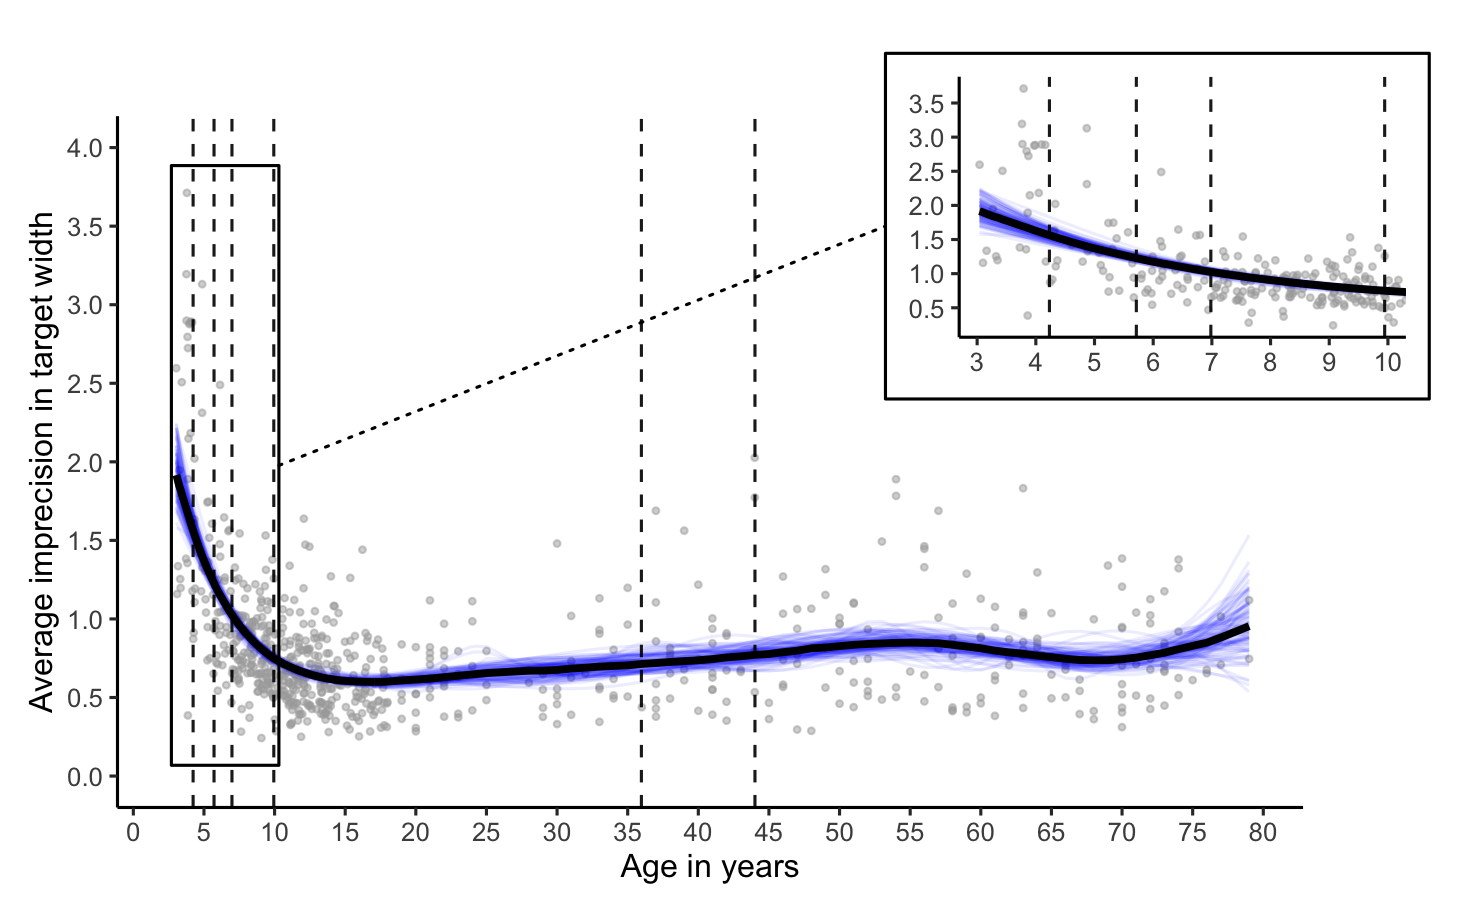
\includegraphics[width=1\linewidth]{../figures/lifespan_plot} \caption{\textbf{Comparison between models on a trial- or subject-level}. Grey dots show data of each trial. Solid lines show the mean predicted developmental trajectory for both models. Line color denotes model structure (yellow: trial-level; black: aggregated on subject-level).}\label{fig:S1}
\end{figure}

\newpage



\begin{figure}[H]
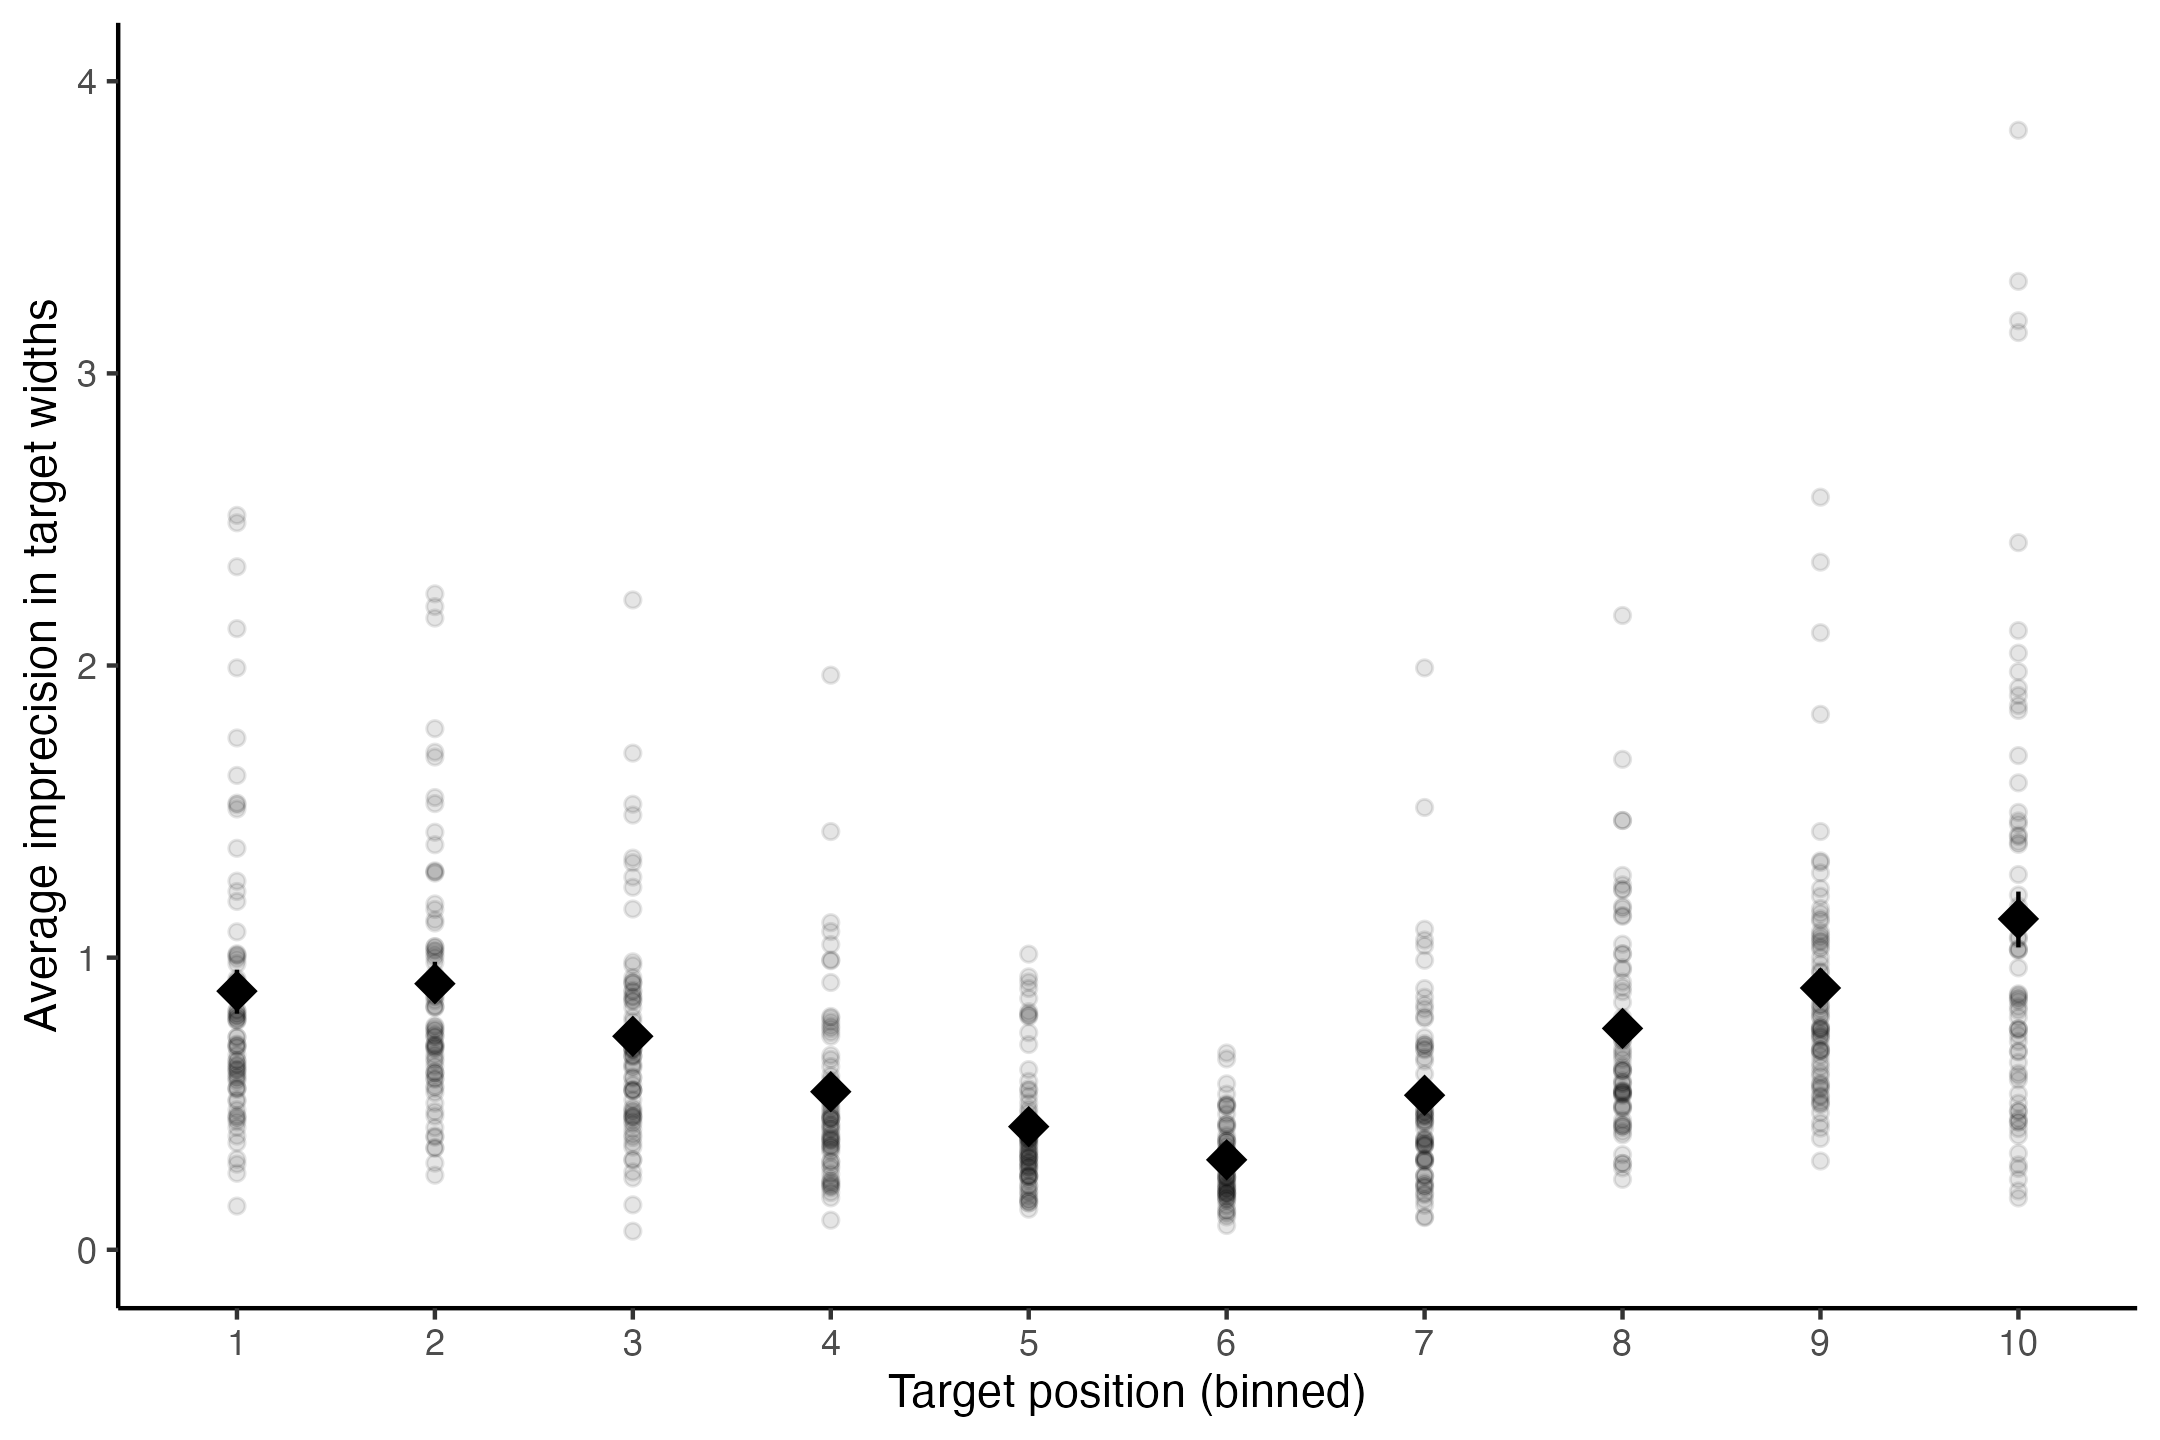
\includegraphics[width=1\linewidth]{../figures/gazefunnel_adults} \caption{\textbf{Gaze funnel for adult sample with higher trial number (30 trials)}. The x-axis shows the target position, binned into 10 sections. The y-axis shows participants' imprecision in target widths.}\label{fig:S2}
\end{figure}

\newpage



\begin{figure}[H]
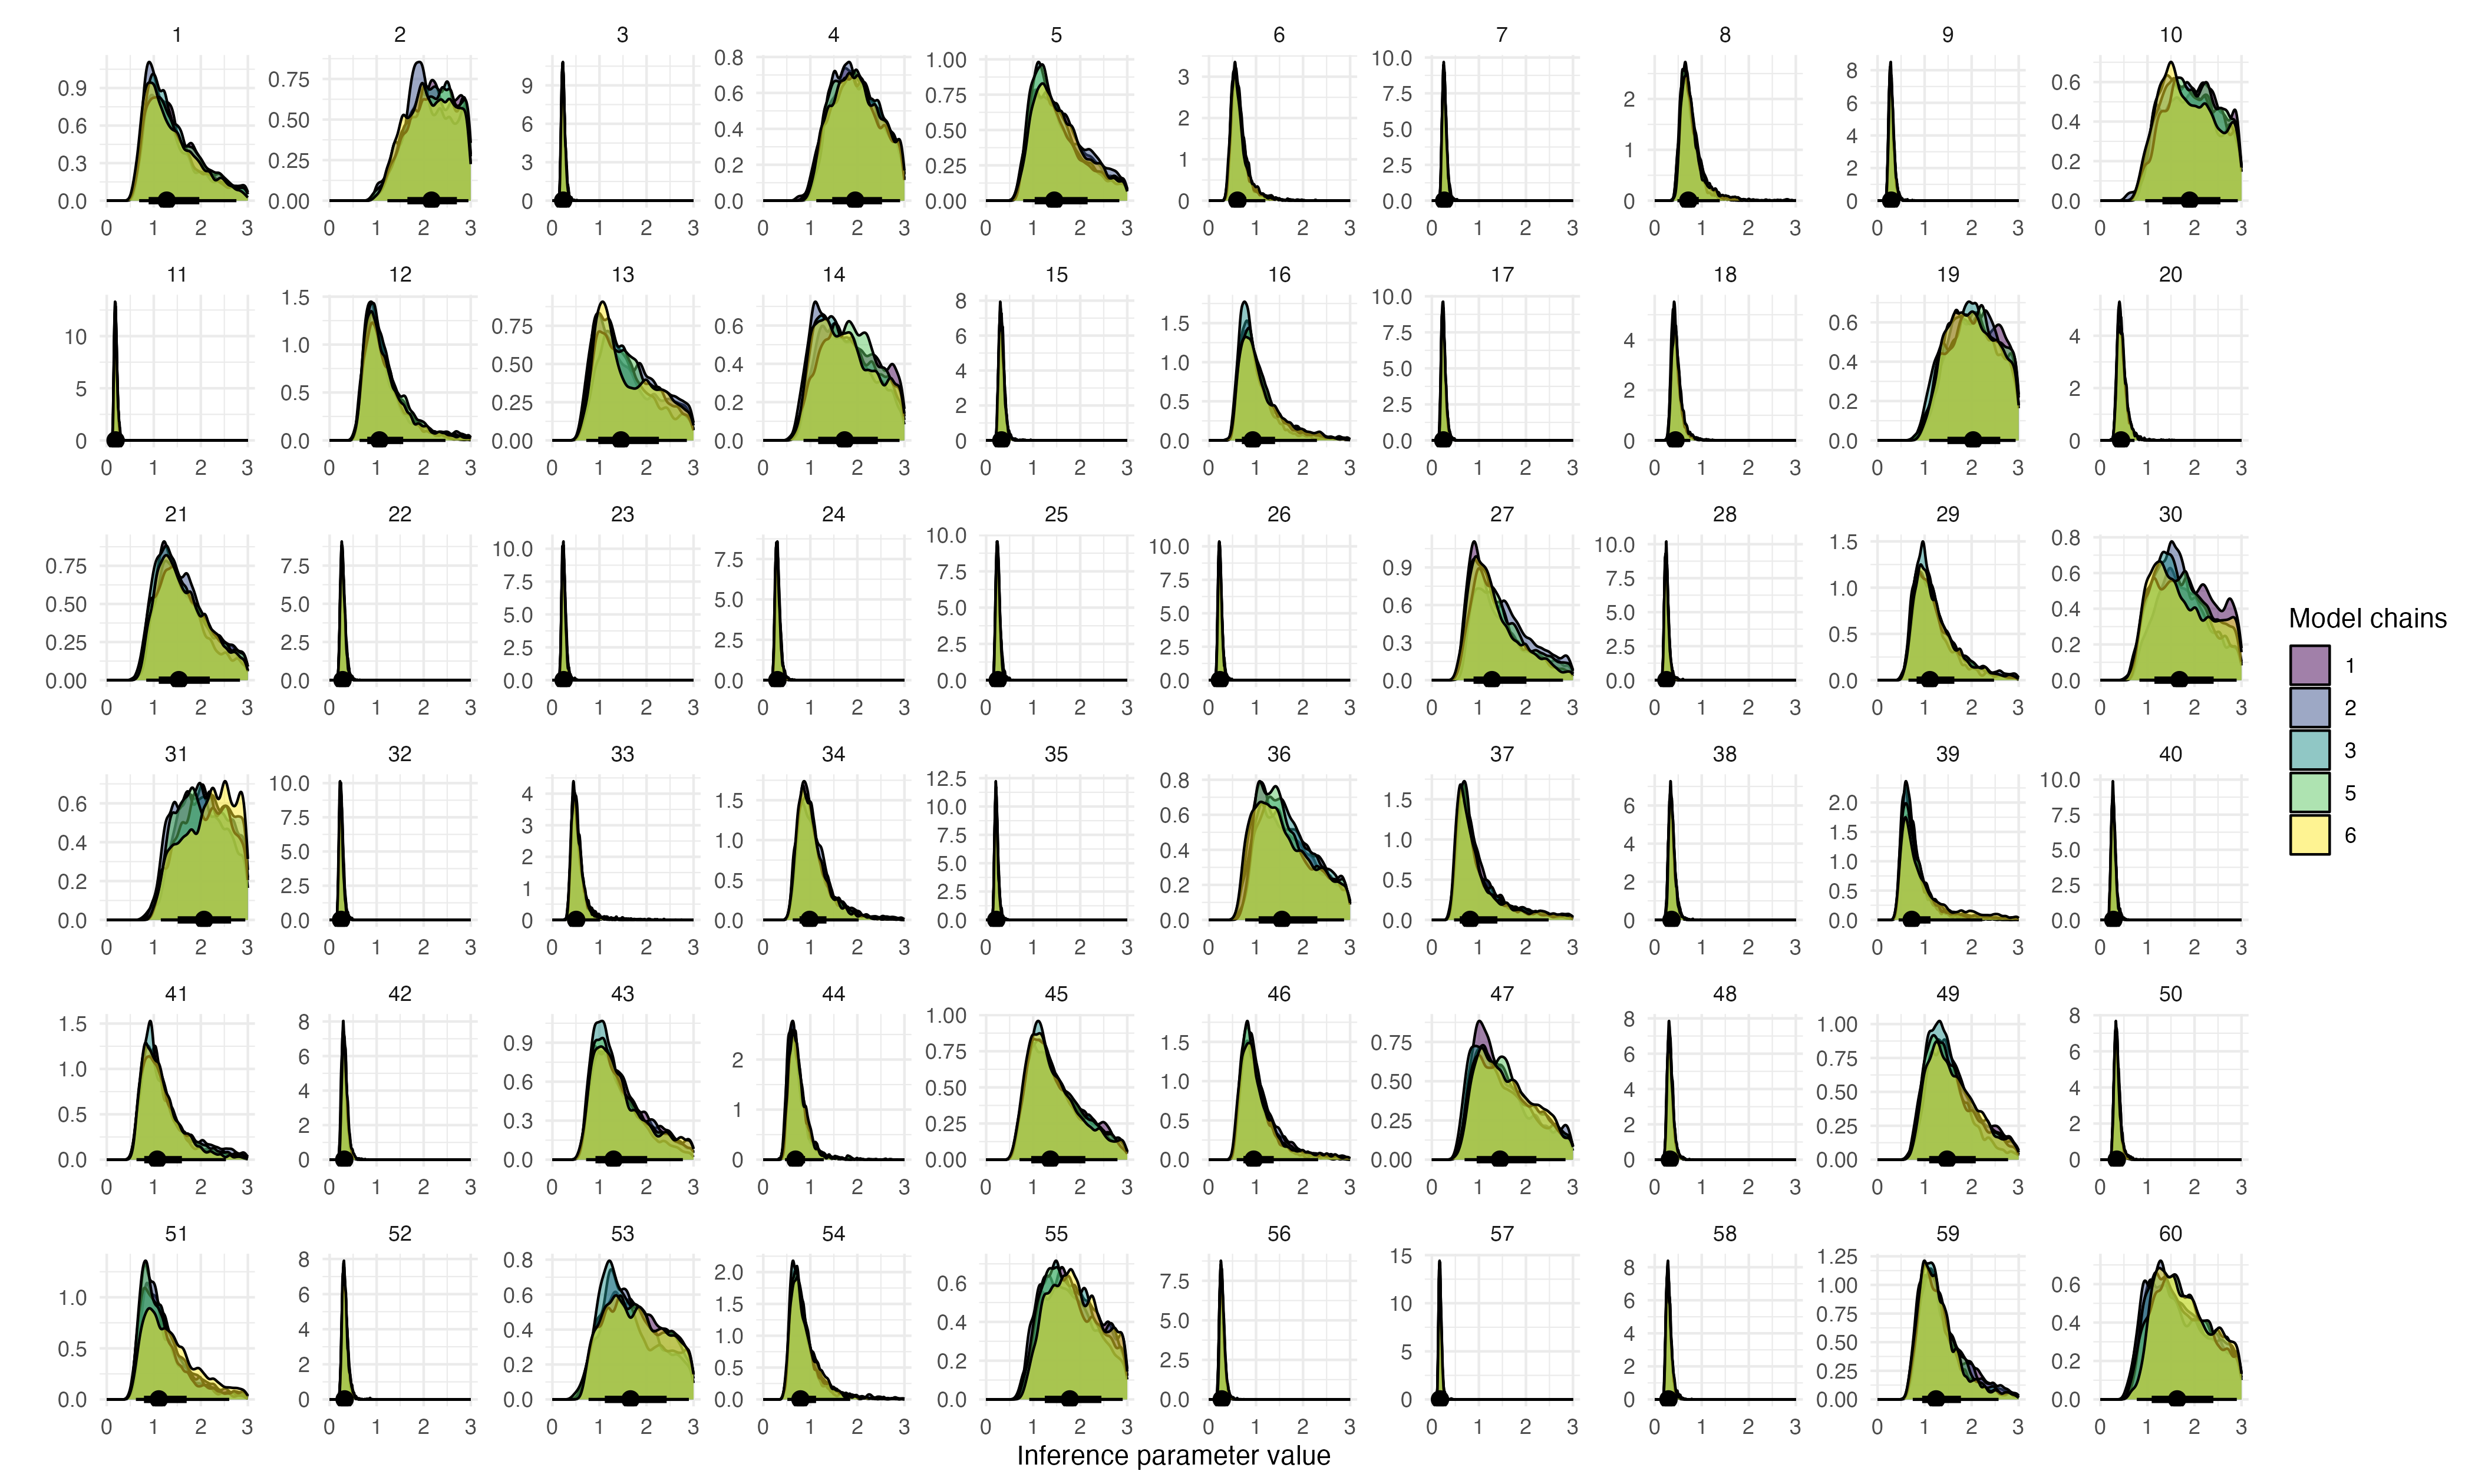
\includegraphics[width=1\linewidth]{../figures/supplements_gazemodel_facetedinference} \caption{\textbf{Gaze model estimates faceted by individual}. Density curves show the distribution of the inference parameter by individual.}\label{fig:S3}
\end{figure}

\newpage



\begin{figure}[H]
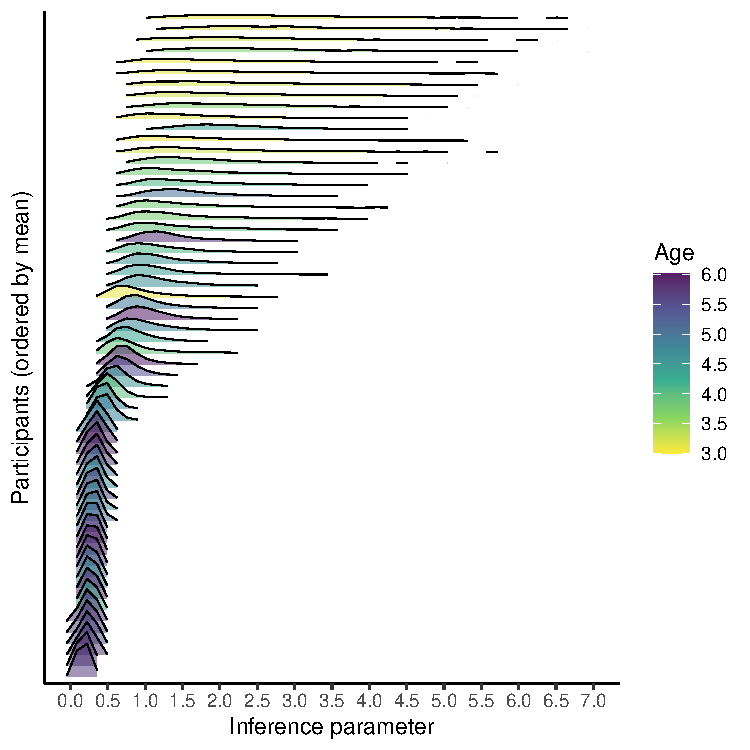
\includegraphics[width=1\linewidth]{../figures/supplements_gazemodel_indinference} \caption{\textbf{Gaze model estimates ordered by descending inference parameter value}. Density curves show the distribution of the inference parameter across individuals.}\label{fig:S4}
\end{figure}

\newpage



\begin{figure}[H]
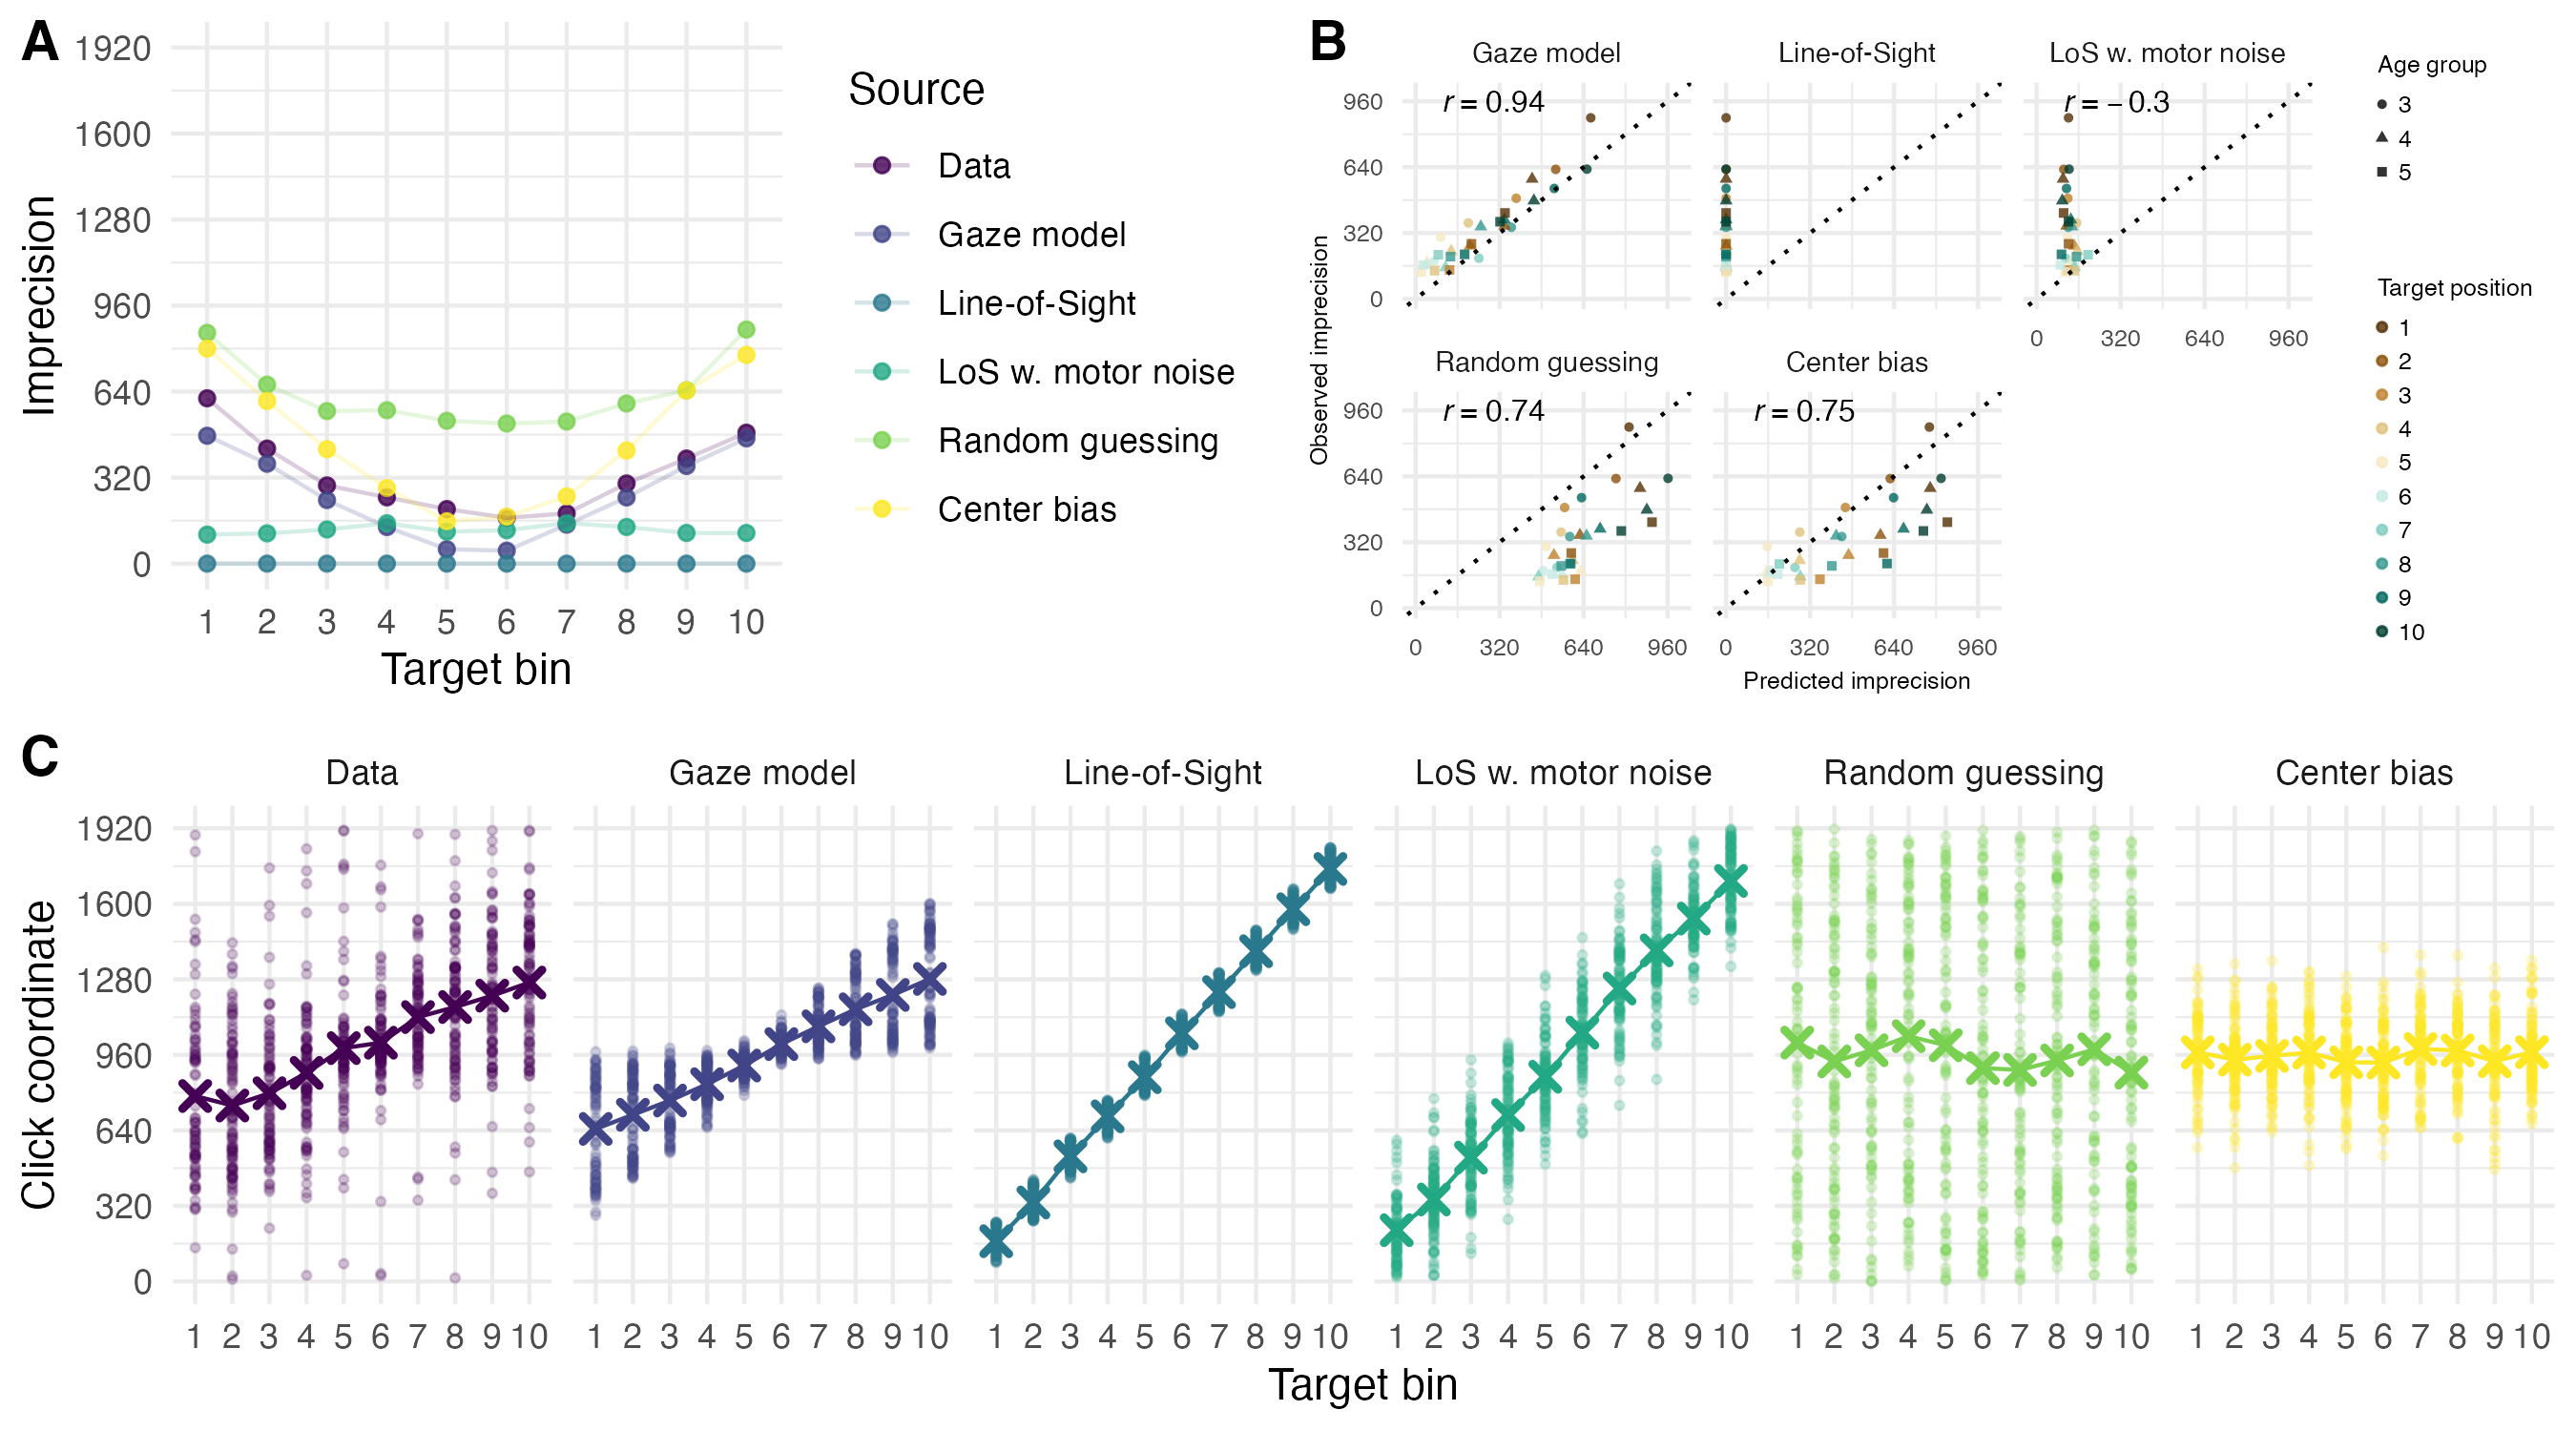
\includegraphics[width=1\linewidth]{../figures/gazemodel_simulated_u} \caption{\textbf{Predictions of alternative models across target positions.} A: Predicted U-pattern across target positions by the different models. Note that this is averaged across trials and displays imprecision, i.e., the absolute distance between the target center and the click. B: Correlation between the predicted imprecision and the observed imprecision, by target position and age group. C: Predicted click coordinates (cf.~not imprecision) by target position across the different models.}\label{fig:S5}
\end{figure}


\clearpage
\renewcommand{\listfigurename}{Figure captions}

\clearpage
\renewcommand{\listtablename}{Table captions}


\end{document}
